% Automatically generated from results/summary.csv. Do not hand-edit values.
% IMPORTANT: estimates are finite-sample Monte Carlo results, not claims of asymptotic optimality.
\section{Simulations}\label{sec:simulations}
We simulated independent $n\times n$ matrices with $X_{ij}\sim N(0,1)$ under the null
and added a positive mean shift $\mu$ to a uniformly sampled, arbitrarily located
$k\times k$ block under the alternative. The block was unknown to each procedure.
All tests used a one-sided nominal level $\alpha=0.05$, with $1{,}500$
independent null samples per configuration to calibrate their rejection
thresholds; the combined sum-or-scan procedure used a Bonferroni split of
$\alpha/2$ between its two component thresholds. We evaluated each configuration
on $600$ independently generated null matrices and $600$ independently generated
alternatives at each signal strength. The tests used paired matrices within
each replicate. We recorded empirical Type I error and detection power, and
reported Wilson $95\%$ confidence intervals for each conditional binomial
proportion. Calibration variability is not included in those intervals.

For exact recovery, we evaluated $600$ independent alternative matrices per
configuration and recorded success only when \emph{both} affected index sets
were recovered exactly. The exhaustive scan and maximizing-block estimator
were computed exactly by enumerating row subsets and optimizing the column
subset for each. Consequently, exhaustive procedures were evaluated only
on small matrices. We used the leading singular vectors for spectral projection;
thresholded spectral projection applied fixed soft thresholding before
computing those vectors. The mean shift grid and threshold choices were
fixed before evaluating test outcomes. All random draws used the seeded
NumPy generator; the exact code, per-trial records and figures are archived
with the project repository.

\begin{table}[t]
\centering\small
\caption{Selected finite-sample simulation results. Each entry is an estimated detection power or exact-recovery probability and its Wilson $95\%$ interval from $600$ replications.}
\begin{tabular}{@{}llcll@{}}\toprule
Configuration & $(n,k)$ & $\mu$ & Procedure & Estimate (95\% CI) \\
\midrule
D1 & $(16,4)$ & $1.2$ & Global sum & $34.3\%\;[30.6,\,38.2]\%$ \\
D1 & $(16,4)$ & $1.2$ & Exhaustive scan & $63.7\%\;[59.7,\,67.4]\%$ \\
D1 & $(16,4)$ & $1.2$ & Maximum entry & $17.3\%\;[14.5,\,20.6]\%$ \\
D3 & $(64,16)$ & $0.6$ & Global sum & $77.8\%\;[74.3,\,81.0]\%$ \\
D3 & $(64,16)$ & $0.6$ & Column pooling & $36.3\%\;[32.6,\,40.3]\%$ \\
D3 & $(64,16)$ & $0.6$ & Maximum entry & $8.3\%\;[6.4,\,10.8]\%$ \\
D4 & $(64,4)$ & $2.5$ & Global sum & $14.3\%\;[11.8,\,17.4]\%$ \\
D4 & $(64,4)$ & $2.5$ & Maximum entry & $50.3\%\;[46.3,\,54.3]\%$ \\
D4 & $(64,4)$ & $2.5$ & Column pooling & $15.2\%\;[12.5,\,18.3]\%$ \\
R1 & $(16,4)$ & $1.75$ & Exhaustive maximizer & $63.2\%\;[59.2,\,66.9]\%$ \\
R1 & $(16,4)$ & $1.75$ & Spectral projection & $44.8\%\;[40.9,\,48.8]\%$ \\
R4 & $(64,4)$ & $3$ & Spectral projection & $74.2\%\;[70.5,\,77.5]\%$ \\
R4 & $(64,4)$ & $3$ & Thresholded spectral & $90.2\%\;[87.5,\,92.3]\%$ \\
\bottomrule\end{tabular}\label{tab:simulation-results}
\end{table}

Figure~\ref{fig:power-curves} compares detection power, while
Figure~\ref{fig:recovery-curves} shows exact-recovery probabilities.
In the $(n,k)=(16,4)$ setting, scanning improves power over the global sum
at moderate shifts, reflecting its ability to concentrate on a sparse block.
For $(64,16)$, aggregation becomes more effective at weak shifts, whereas
for $(64,4)$ the maximum-entry test can outperform global aggregation when
individual signals are large. Exact recovery can require substantially more
signal than simple detection; in the $(64,4)$ example soft-thresholded
spectral projection improves over the unthresholded spectral baseline at
intermediate shifts. These finite-sample comparisons do not establish
computational lower bounds or prove asymptotic phase transitions.

\begin{figure}[t]\centering
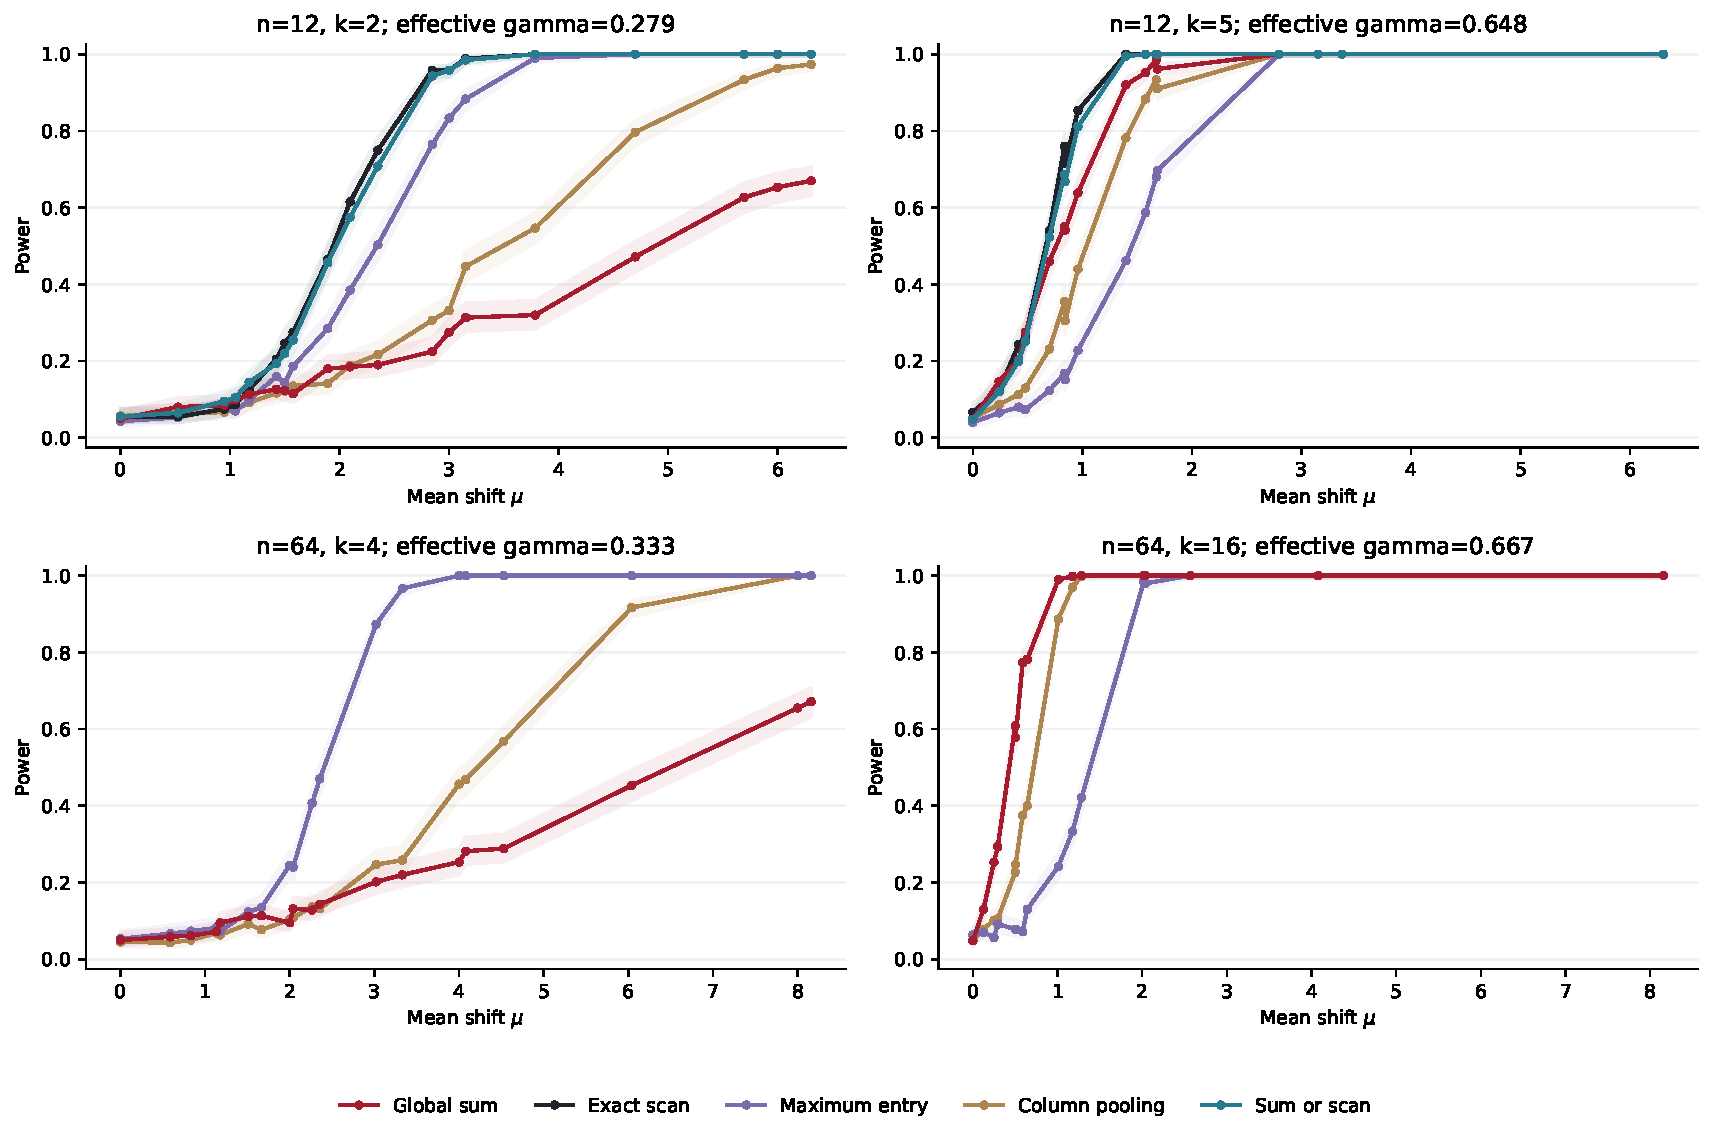
\includegraphics[width=\textwidth]{figures/detection_power.pdf}
\caption{Empirical detection power at nominal level $\alpha=0.05$.
Shaded bands denote marginal Wilson $95\%$ confidence intervals; all
procedures within an experiment are run on paired matrices.}
\label{fig:power-curves}\end{figure}
\begin{figure}[t]\centering
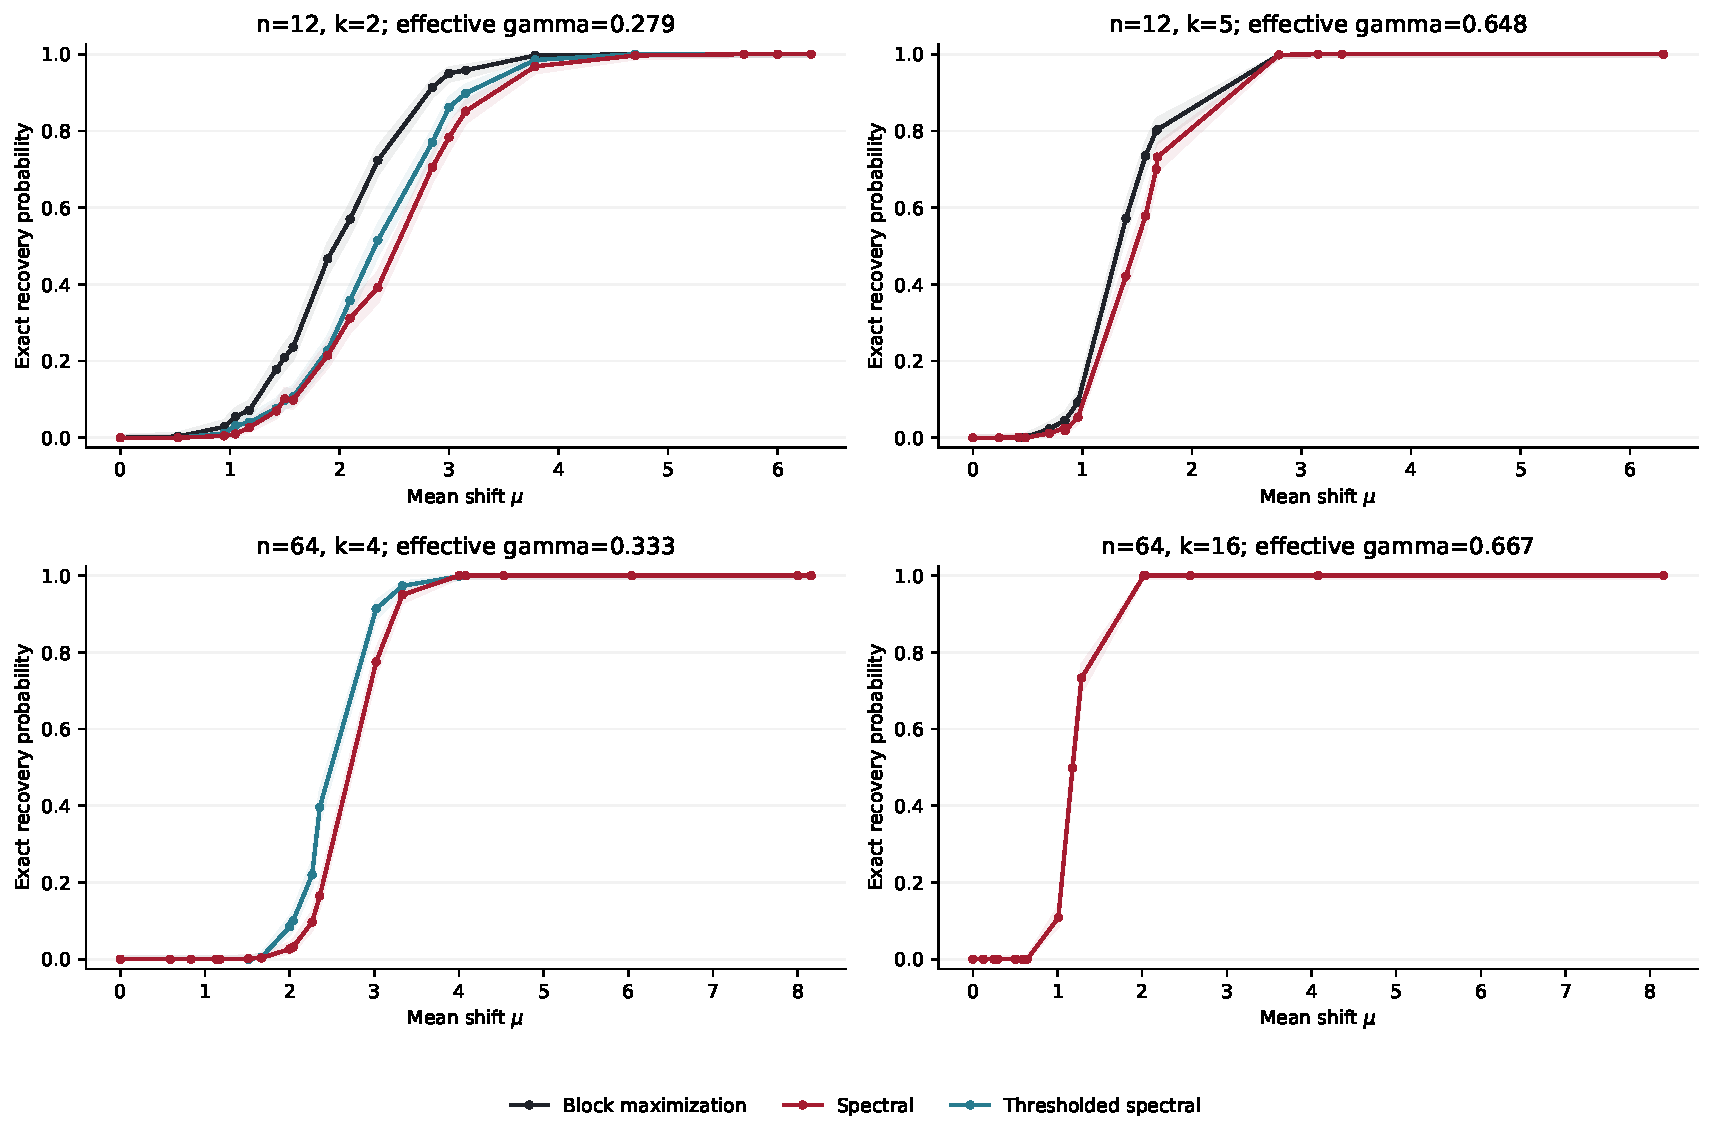
\includegraphics[width=\textwidth]{figures/exact_recovery.pdf}
\caption{Exact recovery probability. An estimate counts as correct only if
both affected row and column index sets match their planted values.}
\label{fig:recovery-curves}\end{figure}